
\documentclass[a4paper,12pt]{article}
\usepackage{graphicx}
%\usepackage{stix}
\usepackage{amsmath}
\newcommand\addtag{\refstepcounter{equation}\tag{\theequation}}
\begin{document}

\title{Diagnosed Particle Disaggregation}
\author{Jacob A. Cram}
\maketitle

\section{Definitions and Units}

\begin{equation}
  m = C_m r^\alpha %\addtag
  \label{eqn:m}
\end{equation}

As in DeVries et al. [2014] particle mass m is a function of radius r and scales with a fractal dimension $\alpha$. $C_m$ is a constant.

\begin{equation}
  w = C_wr^\gamma %\addtag
  \label{eqn:w}
\end{equation}

Sinking speed also scales with mass to another constant $\gamma$. 
According to Guidi et al. [2008] $\gamma = \alpha - 1$, but we'll keep things in terms of $\gamma$ going forward.

\begin{equation}
  F = nmw = n C_m C_w r^{\alpha + \gamma}
\end{equation}

Flux F is a function of particle numbers, mass, and sinking speed.


\begin{figure}[h]

  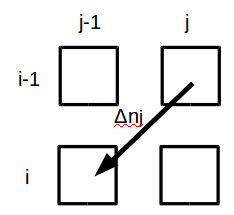
\includegraphics[natwidth=0.35\textwidth]{ijFig2.png}
  
  \centering
  \caption{Some number of particles $\Delta n_j$ of size ``j'' remineralize to size ``j-1'' as they sink from depth ``i-1'' to depth ``i''.}
  \label{fig:boxes}
\end{figure}

Going forward we will determine the calculations for how many particles of size j in shallow depth i-1 remineralize into smaller particles of size j-1 in deeper depth i. We will call this term $\Delta n_j$

\section{Conservation of particle number flux}

In the absence of disaggregation, the number of particles leaving a box of water is equal to the number of particles going into that box from above. In other words, particle "number-flux" is conserved. Thus the number of particles in the box is a function of the number of particles going into that box, and the difference in velocities between when the particle enters and when that particle leaves.

\begin{equation}
n_{i-1, j-1}  {{w_{j-1}}\over{w_j}} + n_{i-1,j} = n_{i,j-1} {{w_{j-1}}\over{w_j}} + n_{i,j}
\label{eqn:nfcons}
\end{equation}

Where $n_{i-1,j}$ is the number of particles of size j (the bigger size) at depth i-1 (the shallower depth). The subscripts correspond to locations in Figure \ref{fig:boxes}.

We can re-arrange equation \ref{eqn:nfcons}

\begin{equation}
n_{i-1, j-1} w_{j-1} + n_{i-1,j} w_j = n_{i,j-1} w_{j-1} + n_{i,j} w_j
\label{eqn:renfcons}
\end{equation}


Substitue in equation \ref{eqn:w} into equation \ref{eqn:renfcons}.

\begin{equation}
n_{i-1, j-1} r^\gamma_{j-1} + n_{i-1,j} r^\gamma_j = n_{i,j-1} r^\gamma_{j-1} + n_{i,j} r^\gamma_j
\label{eqn:nra}
\end{equation}

Rearrange equation \ref{eqn:nra}
\begin{equation}
r^\gamma_{j-1} (n_{i-1, j-1} - n_{i, j-1} ) = r^\gamma_{j} (n_{i, j} - n_{i-1, j} ) = \Phi
\label{eqn:phi}
\end{equation}

Where $\Phi$ is a placeholder standing for either side of equation \ref{eqn:phi}, which I will subsequently substitute into things.

\medskip

Solve for $\Delta n_j$
 \begin{equation}
\Delta n_j = n_{i, j} - n_{i-1, j} = {{r^\gamma_{j-1}}\over{r^\gamma_{j}}} (n_{i-1,j-1}-n_{i,j-1})
 \end{equation}

\section{Conservation of Mass Flux}

Total flux defined is the sum of flux in each (observed) particle size bin. Particles not in an observed bin don't count towards total flux.

\begin{equation}
\Delta F = \sum_{j = 2}^n \Delta f_j + \Delta f_1
\label{eqn:df}
\end{equation}

Here $\Delta f_j$ is the flux attenuation from bin of size j and $\Delta f_1$ is the loss that comes from particles in bin 1 becoming small enough that you can no longer see them with the UVP.

The flux attenuation in a bin is the product of the rate of flux attenuation with depth of each individual particle ${\partial f} \over {\partial z}$, the depth interval over which the particles attenuate $\Delta z$ and the number of particles in that bin at the top of the depth interval $n_{i-1,j}$

\begin{equation}
\Delta f_j = {{\partial f} \over {\partial z}} \Delta z n_{i-1,j}
\label{eqn:dfj}
\end{equation}

Furthermore, the rate of flux attenuation with respect to depth is the product of the rate of mass attenuation with respect to time ${{\partial m} \over {\partial t}}$ , the inverse of the sinking speed ${{\partial t} \over {\partial z}}$ , and the deriviative of the flux to mass relationship ${{\partial f} \over {\partial m}}$.

\begin{equation}
{{\partial f} \over {\partial z}} = 
{{\partial m} \over {\partial z}} {{\partial f} \over {\partial m}} = 
{{\partial m} \over {\partial t}} 
{{\partial t} \over {\partial z}} 
{{\partial f} \over {\partial m}}
\label{eqn:dfdz}
\end{equation}

In PRiSM, fractional mass loss as a function of time is the same for all particles of all sizes.

\medskip

Now we are going to come up with the values for each of these terms.

\medskip

The particle remineralization rate $C_r$ is the same for particles of all sizes.

\begin{equation}
{{\partial m} \over {\partial t}} = C_r * m = C_r  C_m r^\alpha
\label{eqn:dmdt}
\end{equation}

Sinking speed definition, substituting from equation \ref{eqn:w}
\begin{equation}
{{\partial t} \over {\partial z}} = {1 \over w} = {1 \over C_w r^\gamma}
\label{eqn:dtdz}
\end{equation}

Flux for a given size class, substituting eqation \ref{eqn:m}, and finally putting everything in terms of mass (rather than mass and radius, since the two are related)
\begin{equation}
f = m w = m * C_w r^\gamma = m * C_w ({m\over C_m})^{\gamma \over \alpha}
\label{eqn:f}
\end{equation}

Derriving equation \ref{eqn:f} with respect to mass, and substituting equation \ref{eqn:m}
\begin{equation}
{{\partial f} \over {\partial m}} = 
Cw(1+{\gamma \over \alpha}) ({m \over C_m}) ^ {\gamma \over \alpha}=
C_w(1+{\gamma \over \alpha}) r ^ \gamma
\label{eqn:dfdm}
\end{equation}

Finally, we can construct our equation for flux attenuation by substituting equations \ref{eqn:dmdt}, \ref{eqn:dtdz} and \ref{eqn:dfdm} into equation \ref{eqn:dfdz}

\begin{equation}
{{\partial f} \over {\partial z}} = C_r C_m r^\alpha(1+{\gamma \over \alpha})
\end{equation}


And now we can solve for equation \ref{eqn:dfj}.

\begin{equation}
\Delta f_j = C_r C_m r^\alpha (1+{\gamma \over \alpha}) \Delta z * n_{i-1,j}
\label{eqn:dfj}
\end{equation}

We also need to solve for $\Delta f_1$ the flux ``attenuation'' that actually comes from particles leaving the smallest bin and escaping from what the UVP sees.

\begin{equation}
\Delta f_1 = \Delta n_1 m_1 w_1 =  \Delta n_1 C_m C_w r_1^{\alpha + \gamma}
\label{eqn:df0}
\end{equation}

Here, $\Delta n_1$ is the number of particles leaving bin j = 1, but we haven't solved for that yet.

\section{Solving for $\Delta n_j$}

Recall that $\Delta n_j$ is the number of particles that migrate between bin ``j'' and bin ``j-1'' as the particles sink from depth ``i-1'' to depth ``i''.

The flux at the shallower depth is equal to the flux at the deeper depth, plus the flux that attenuated between those two depths. Since $f = nmw$ and we know m and w

\begin{equation}
n_{i-1,j-1} C_m C_w r_{j-1}^{\alpha + \gamma} + n_{i-1,j} C_m C_w r_{j}^{\alpha + \gamma} =
n_{i,j-1} C_m C_w r_{j-1}^{\alpha + \gamma} + n_{i,j} C_m C_w r_{j}^{\alpha + \gamma} + \Delta f_j
\label{eqn:n4f}
\end{equation}

This equation can be re-arranged, and we can substitute in equation \ref{eqn:dfj} for $\Delta f_j$. 
 
% \begin{equation}
% C_m C_w r_{j-1} ^{\alpha + \gamma} (n_{i-1,j-1}- n_{i,j-1}) = 
% C_m C_w r_{j}^{\alpha + \gamma} (n_{i,j} - n_{i-1,j}) +  C_r C_m (1 + {\gamma \over \alpha}) \Delta z n_{i-1,j} r ^ \alpha
% \end{equation}

The $C_m$ cancel out.

\begin{equation}
 C_w r_{j-1} ^{\alpha + \gamma} (n_{i-1,j-1}- n_{i,j-1}) = 
 C_w r_{j}^{\alpha + \gamma} (n_{i,j} - n_{i-1,j}) +  C_r  (1 + {\gamma \over \alpha}) \Delta z n_{i-1,j} r ^ \alpha
\end{equation}

We can then substitute in $\Phi$ from equation \ref{eqn:phi}.
\begin{equation}
C_w r_{j-1} ^{\alpha} \Phi = 
 C_w r_{j}^{\alpha} \Phi +  C_r  (1 + {\gamma \over \alpha}) \Delta z n_{i-1,j} r ^ \alpha
\end{equation}


Rearrange
% C_w \Phi %(r_{j-1}^\alpha - r_j^\alpha)

\begin{equation}
C_w\Phi(r_{j-1}^\alpha - r_j^\alpha) = Cr(1 + {\gamma \over \alpha}) \Delta z r^{\alpha} n_{i-1,j}
\end{equation}

solve for $\Phi$

\begin{equation}
\Phi = {{{C_r \over C_w} \Delta z r^{\alpha} n_{i-1,j}(1 + {\gamma \over \alpha})} \over {r_{j-1}^\alpha - r_j^\alpha}}
\end{equation}

\begin{equation}
\Delta n_j = {\Phi \over r_j^\gamma} = {{{C_r \over C_w} \Delta z r^{\alpha} n_{i-1,j}(1 + {\gamma \over \alpha})} \over {r_j^\gamma(r_{j-1}^\alpha - r_j^\alpha})}
\label{eqn:dnj}
\end{equation}

\begin{equation}
\Delta n_{j-1} = {\Phi \over r_{j-1}^\gamma} = {{\Delta n_j r_j^\gamma} \over {r_{j-1}^\gamma}}
\end{equation}

At this point, the only unsolved variable is $C_r$, which we can now calculate.


\section{Solving for $C_r$}

We can calculate $\Delta F $, the attenuation of flux and can impose the size spectrum and all of the other constants. Here we find the $C_r$ that gives us the correct $\Delta F $

First, to solve equation \ref{eqn:df} by substituting in equaitons \ref{eqn:dfj} and \ref{eqn:df0}

\begin{equation}
\Delta F = \sum_{j = 2}^n \Delta f_j + \Delta f_1 = 
\sum_{j = 2}^n \left\{C_r C_m r_j^\alpha(1+{\gamma \over \alpha}) \Delta z n_{i-1,j} \right\} +
\Delta n_1 C_m C_w r_1^{\alpha + \gamma}
\end{equation}

Substitute equation \ref{eqn:dnj} for $\Delta n_j$ when j = 1 for $\Delta n_1$

\begin{equation}
\Delta F = \sum_{j = 2}^n \Delta f_j + \Delta f_1 = 
\sum_{j = 2}^n \left\{C_r C_m r_j^\alpha(1+{\gamma \over \alpha}) \Delta z n_{i-1,j} \right\} +
 {{{C_r \over C_w} \Delta z r_1^{\alpha} n_{i-1,1}(1 + {\gamma \over \alpha})} \over {r_1^{\gamma}(r_{0}^\alpha - r_1^\alpha})}
C_m C_w r_1^{\alpha + \gamma}
\end{equation}

In the above, $r_0$ is the effective size of the particles smaller than the UVP can see. In principle this is arbitrary. Numbers closer to zero result in fewer particles in the smallest bin disapearing, larger ones to more of those particles disapearing. As $r_0$ approaches $r_1$ Cr approaches zero. They cannot be equal or the math breaks.

Pull what I can out of the sum operation, and cancel out $r^{\gamma}$ and $C_w$ from the rightmost term
\begin{equation}
\Delta F =
C_r C_m \Delta z (1 + {\gamma \over \alpha}) \sum_{j = 2}^n \left\{r_j^\alpha n_{i-1,j} \right\}
+
 {{{C_r} \Delta z r_1^{2 \alpha} n_{i-1,1}(1 + {\gamma \over \alpha})} \over {(r_{0}^\alpha - r_1^\alpha})}
C_m 
\end{equation}

Now we can solve for $C_r$

\begin{equation}
C_r = {
\Delta F \over 
C_m \Delta z 
(1 + {\gamma \over \alpha}) \big[ \sum_{j = 2}^n  \big\{
r_j^\alpha n_{i-1,j}
\big\} +
{{r_1^{2\alpha}n_{i-1,1}}\over{r_0^\alpha - r_1^\alpha}}
\big]
}
\end{equation}

Thus for a pair of profiles, we can estemate the flux attenuation, calculate Cr from that, and then plug Cr (and the profile) into the equation \ref{eqn:dnj} for $\Delta n_j$. We can thus compute $\Delta n_j$ for each size class to see how many particles from that bin move to the next bin smaller.



 \end{document}


